\documentclass[12pt,a4paper]{article}
\usepackage[utf8]{vietnam}
\usepackage{amsmath,amssymb}
\usepackage[a4paper,left=2cm,right=1.8cm,top=1.8cm,bottom=1.8cm]{geometry}
\usepackage{tikz}
\usepackage{array,tabularx,longtable}
\usepackage{enumitem}
\setlength{\parindent}{0pt}
\setlength{\parskip}{3pt}
\linespread{1.15}
\pagestyle{plain}

% Phương án trắc nghiệm: 4 phương án trên 1 dòng / 2 dòng / mỗi phương án 1 dòng
\newcommand{\bonpa}[4]{\par\noindent\begin{tabularx}{\linewidth}{@{\hspace{0.6cm}}XXXX@{}}
\textbf{A.} #1 & \textbf{B.} #2 & \textbf{C.} #3 & \textbf{D.} #4\end{tabularx}\par}
\newcommand{\haipa}[4]{\par\noindent\begin{tabularx}{\linewidth}{@{\hspace{0.6cm}}XX@{}}
\textbf{A.} #1 & \textbf{B.} #2\\ \textbf{C.} #3 & \textbf{D.} #4\end{tabularx}\par}
\newcommand{\motpa}[4]{\par\hspace*{0.6cm}\textbf{A.} #1\par\hspace*{0.6cm}\textbf{B.} #2\par
\hspace*{0.6cm}\textbf{C.} #3\par\hspace*{0.6cm}\textbf{D.} #4\par}
\newcommand{\cau}[1]{\par\medskip\textbf{Câu #1.}~}
\newcommand{\bai}[2]{\par\medskip\textbf{Bài #1} \textit{(#2)}.~}
\newcommand{\y}[1]{\par\hspace*{0.6cm}#1}
\newcommand{\phan}[1]{\par\bigskip{\large\textbf{#1}}\par\smallskip}
\setlength{\extrarowheight}{2pt}

\begin{document}
% ===================== ĐỀ SỐ 2 =====================
\noindent
\begin{minipage}[t]{0.38\linewidth}\centering
TRƯỜNG THCS \dotfill\\[2pt]
\textbf{ĐỀ SỐ 2}
\end{minipage}\hfill
\begin{minipage}[t]{0.6\linewidth}\centering
\textbf{ĐỀ KIỂM TRA GIỮA HỌC KÌ I}\\
\textbf{NĂM HỌC 2026 -- 2027}\\
\textbf{MÔN: TOÁN 7} -- Sách \textit{Kết nối tri thức với cuộc sống}\\
\textit{Thời gian làm bài: 90 phút (không kể thời gian giao đề)}
\end{minipage}

\medskip
Họ và tên: \dotfill\ Lớp: \makebox[2cm]{\dotfill}\ Số báo danh: \makebox[2.5cm]{\dotfill}
\phan{A. TRẮC NGHIỆM (3,0 điểm)}
\textbf{Phần I. Câu trắc nghiệm nhiều phương án lựa chọn} \textit{(1,0 điểm)}. Thí sinh trả lời từ câu 1 đến câu 4. Mỗi câu hỏi thí sinh chỉ chọn một phương án.
\cau{1} Số đối của số hữu tỉ $-\dfrac{5}{7}$ là
\bonpa{$\dfrac{5}{7}$}{$-\dfrac{5}{7}$}{$\dfrac{7}{5}$}{$-\dfrac{7}{5}$}
\cau{2} Với $x$ là số hữu tỉ khác $0$, kết quả của phép tính $x^{5}\cdot x^{3}$ là
\bonpa{$x^{15}$}{$x^{8}$}{$x^{2}$}{$2x^{8}$}
\cau{3} Phân số $\dfrac{1}{3}$ được viết dưới dạng số thập phân là
\bonpa{$0{,}3$}{$0{,}(3)$}{$0{,}33$}{$3{,}(3)$}
\cau{4} Nếu một đường thẳng cắt hai đường thẳng song song thì hai góc so le trong
\bonpa{bằng nhau.}{bù nhau.}{phụ nhau.}{kề bù.}

\medskip\textbf{Phần II. Câu trắc nghiệm đúng sai} \textit{(1,0 điểm)}. Trong mỗi ý a), b), c), d) ở câu 5, thí sinh chọn đúng hoặc sai.
\cau{5} Cho $\widehat{xOy}=80^\circ$, tia $Ot$ là tia phân giác của $\widehat{xOy}$. Vẽ tia $Ox'$ là tia đối của tia $Ox$.
\y{a) $\widehat{xOt}=40^\circ$.}
\y{b) $\widehat{x'Oy}=100^\circ$.}
\y{c) $\widehat{x'Ot}=150^\circ$.}
\y{d) $\widehat{xOy}$ và $\widehat{x'Oy}$ là hai góc đối đỉnh.}

\medskip\textbf{Phần III. Câu trắc nghiệm trả lời ngắn} \textit{(1,0 điểm)}. Thí sinh trả lời từ câu 6 đến câu 9.
\cau{6} Tính giá trị của biểu thức $\left(-\dfrac{1}{3}\right)^{2}\cdot 27$.
\cau{7} Tìm $x$, biết $\dfrac{x}{4}=-\dfrac{3}{2}$.
\cau{8} Cho tam giác $ABC$ vuông tại $A$ có $\widehat{B}=35^\circ$. Tính số đo $\widehat{C}$ (đơn vị: độ).
\cau{9} Cho $\triangle ABC=\triangle DEF$, biết $AB=5$ cm, $BC=7$ cm, $DF=6$ cm. Tính chu vi tam giác $DEF$ (đơn vị: cm).
\phan{B. TỰ LUẬN (7,0 điểm)}
\bai{1}{1,0 điểm} Tính (hợp lí nếu có thể):
\par\noindent\begin{tabularx}{\linewidth}{@{\hspace{0.6cm}}XX@{}}a) $\dfrac{-7}{13}\cdot\dfrac{5}{11}+\dfrac{-7}{13}\cdot\dfrac{6}{11}+1\dfrac{7}{13}$; & b) $\left(\dfrac{2}{3}\right)^{3}\cdot\left(\dfrac{3}{2}\right)^{2}-\dfrac{1}{3}$.\end{tabularx}
\bai{2}{1,5 điểm} Tìm $x$, biết:
\y{a) $\dfrac{2}{5}x=-\dfrac{4}{15}$;}
\y{b) $\dfrac{1}{2}-\left(x+\dfrac{1}{3}\right)=\dfrac{3}{4}$;}
\y{c) $2^{x}+2^{x+2}=40$.}
\bai{3}{1,0 điểm} Lớp 7A có $40$ học sinh. Số học sinh xếp loại Tốt chiếm $\dfrac{1}{4}$ số học sinh cả lớp. Số học sinh xếp loại Khá bằng $\dfrac{3}{5}$ số học sinh còn lại, các học sinh còn lại xếp loại Đạt. Tính số học sinh mỗi loại của lớp 7A.
\bai{4}{1,5 điểm} Cho hình vẽ bên, biết $Ax\parallel By$, $\widehat{xAO}=40^\circ$, $\widehat{OBy}=30^\circ$. Vẽ tia $Ot$ nằm trong $\widehat{AOB}$ sao cho $Ot\parallel Ax$.
\begin{center}
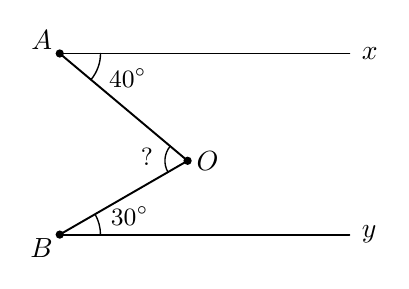
\begin{tikzpicture}[scale=1.15,line cap=round,line join=round]
  \draw[line width=0.7pt] (0.000,2.000) -- (3.200,2.000);
  \draw[line width=0.7pt] (0.000,0.000) -- (3.200,0.000);
  \draw[line width=0.7pt] (0.000,2.000) -- (1.412,0.815);
  \draw[line width=0.7pt] (0.000,0.000) -- (1.412,0.815);
  \node[anchor=west,inner sep=1pt] at (3.300,2.000) {$x$};
  \node[anchor=west,inner sep=1pt] at (3.300,0.000) {$y$};
  \fill (0.000,2.000) circle (1.3pt);
  \node[anchor=center,inner sep=1pt] at (-0.200,2.150) {$A$};
  \fill (0.000,0.000) circle (1.3pt);
  \node[anchor=center,inner sep=1pt] at (-0.200,-0.150) {$B$};
  \fill (1.412,0.815) circle (1.3pt);
  \node[anchor=center,inner sep=1pt] at (1.632,0.815) {$O$};
  \draw[line width=0.5pt] (0.345,1.711) arc[start angle=-40,end angle=0,radius=0.450];
  \node[anchor=center,inner sep=1pt] at (0.752,1.726) {{\small $40^\circ$}};
  \draw[line width=0.5pt] (0.450,0.000) arc[start angle=0,end angle=30,radius=0.450];
  \node[anchor=center,inner sep=1pt] at (0.773,0.207) {{\small $30^\circ$}};
  \draw[line width=0.5pt] (1.220,0.976) arc[start angle=140,end angle=210,radius=0.250];
  \node[anchor=center,inner sep=1pt] at (0.964,0.854) {{\small ?}};
\end{tikzpicture}
\end{center}
\y{a) Chứng minh $Ot\parallel By$.}
\y{b) Tính số đo $\widehat{AOB}$.}
\y{c) Vẽ tia $Om$ là tia phân giác của $\widehat{AOB}$. Tính số đo $\widehat{mOt}$.}
\bai{5}{1,5 điểm} Cho $\widehat{xOy}$ nhọn. Trên tia $Ox$ lấy điểm $A$, trên tia $Oy$ lấy điểm $B$ sao cho $OA=OB$. Lấy điểm $C$ nằm trong $\widehat{xOy}$ sao cho $CA=CB$.
\y{a) Chứng minh $\triangle OAC=\triangle OBC$.}
\y{b) Chứng minh $OC$ là tia phân giác của $\widehat{xOy}$.}
\y{c) Biết $\widehat{xOy}=60^\circ$ và $\widehat{OAC}=100^\circ$. Tính số đo $\widehat{OCB}$.}
\bai{6}{0,5 điểm} So sánh $2^{300}$ và $3^{200}$.

\bigskip\begin{center}\textbf{--------- HẾT ---------}\\
\textit{Giáo viên coi kiểm tra không giải thích gì thêm.}\end{center}

\newpage
\begin{center}{\large\textbf{HƯỚNG DẪN CHẤM -- ĐỀ SỐ 2}}\end{center}
\phan{A. TRẮC NGHIỆM (3,0 điểm)}
\textbf{Phần I.} Mỗi câu trả lời đúng được 0,25 điểm.

\begin{tabular}{|l|*{4}{>{\centering\arraybackslash}p{2cm}|}}\hline
Câu & 1 & 2 & 3 & 4 \\ \hline
Đáp án & \textbf{A} & \textbf{B} & \textbf{B} & \textbf{A} \\ \hline
\end{tabular}

\textbf{Phần II.} Mỗi ý trả lời đúng được 0,25 điểm.

\begin{tabular}{|l|*{4}{>{\centering\arraybackslash}p{2cm}|}}\hline
Câu 5 & a) & b) & c) & d) \\ \hline
Đáp án & \textbf{Đúng} & \textbf{Đúng} & \textbf{Sai} & \textbf{Sai} \\ \hline
\end{tabular}

\textbf{Phần III.} Mỗi câu trả lời đúng được 0,25 điểm.

\begin{tabular}{|l|*{4}{>{\centering\arraybackslash}p{2cm}|}}\hline
Câu & 6 & 7 & 8 & 9 \\ \hline
Đáp án & \textbf{3} & \textbf{$-$6} & \textbf{55} & \textbf{18} \\ \hline
\end{tabular}

\phan{B. TỰ LUẬN (7,0 điểm)}
\begin{longtable}{|>{\bfseries}c|p{0.76\linewidth}|>{\centering\arraybackslash}p{1.3cm}|}\hline
Bài & \multicolumn{1}{c|}{\textbf{Nội dung}} & \textbf{Điểm} \\ \hline\endhead
1a & \rule{0pt}{4ex}$\dfrac{-7}{13}\cdot\left(\dfrac{5}{11}+\dfrac{6}{11}\right)+1\dfrac{7}{13}=\dfrac{-7}{13}\cdot 1+\dfrac{20}{13}$\rule[-2.4ex]{0pt}{0pt} & 0,25 \\ \hline
 & \rule{0pt}{4ex}$=\dfrac{13}{13}=1$\rule[-2.4ex]{0pt}{0pt} & 0,25 \\ \hline
1b & \rule{0pt}{4ex}$\dfrac{8}{27}\cdot\dfrac{9}{4}-\dfrac{1}{3}=\dfrac{2}{3}-\dfrac{1}{3}$\rule[-2.4ex]{0pt}{0pt} & 0,25 \\ \hline
 & \rule{0pt}{4ex}$=\dfrac{1}{3}$\rule[-2.4ex]{0pt}{0pt} & 0,25 \\ \hline
2a & \rule{0pt}{4ex}$x=-\dfrac{4}{15}:\dfrac{2}{5}=-\dfrac{4}{15}\cdot\dfrac{5}{2}$\rule[-2.4ex]{0pt}{0pt} & 0,25 \\ \hline
 & \rule{0pt}{4ex}$x=-\dfrac{2}{3}$. Vậy $x=-\dfrac{2}{3}$.\rule[-2.4ex]{0pt}{0pt} & 0,25 \\ \hline
2b & \rule{0pt}{4ex}$x+\dfrac{1}{3}=\dfrac{1}{2}-\dfrac{3}{4}=-\dfrac{1}{4}$\rule[-2.4ex]{0pt}{0pt} & 0,25 \\ \hline
 & \rule{0pt}{4ex}$x=-\dfrac{1}{4}-\dfrac{1}{3}=-\dfrac{7}{12}$. Vậy $x=-\dfrac{7}{12}$.\rule[-2.4ex]{0pt}{0pt} & 0,25 \\ \hline
2c & $2^{x}+2^{x}\cdot 2^{2}=40$ hay $2^{x}\cdot(1+4)=40$, suy ra $2^{x}=8$ & 0,25 \\ \hline
 & $2^{x}=2^{3}$ nên $x=3$. Vậy $x=3$. & 0,25 \\ \hline
3 & \rule{0pt}{4ex}Số học sinh xếp loại Tốt: $40\cdot\dfrac{1}{4}=10$ (học sinh).\rule[-2.4ex]{0pt}{0pt} & 0,25 \\ \hline
 & Số học sinh còn lại: $40-10=30$ (học sinh). & 0,25 \\ \hline
 & \rule{0pt}{4ex}Số học sinh xếp loại Khá: $30\cdot\dfrac{3}{5}=18$ (học sinh).\rule[-2.4ex]{0pt}{0pt} & 0,25 \\ \hline
 & Số học sinh xếp loại Đạt: $30-18=12$ (học sinh). & 0,25 \\ \hline
4a & Ta có $Ot\parallel Ax$ và $Ax\parallel By$ & 0,25 \\ \hline
 & nên $Ot\parallel By$ (hai đường thẳng phân biệt cùng song song với đường thẳng thứ ba). & 0,25 \\ \hline
4b & Vì $Ot\parallel Ax$ nên $\widehat{AOt}=\widehat{xAO}=40^\circ$ (so le trong); vì $Ot\parallel By$ nên $\widehat{tOB}=\widehat{OBy}=30^\circ$ (so le trong). & 0,25 \\ \hline
 & Tia $Ot$ nằm giữa hai tia $OA$, $OB$ nên $\widehat{AOB}=\widehat{AOt}+\widehat{tOB}=40^\circ+30^\circ=70^\circ$. & 0,25 \\ \hline
4c & \rule{0pt}{4ex}$Om$ là tia phân giác của $\widehat{AOB}$ nên $\widehat{AOm}=\dfrac{70^\circ}{2}=35^\circ$.\rule[-2.4ex]{0pt}{0pt} & 0,25 \\ \hline
 & Vì $\widehat{AOm}<\widehat{AOt}$ nên tia $Om$ nằm giữa hai tia $OA$, $Ot$; suy ra $\widehat{mOt}=40^\circ-35^\circ=5^\circ$. & 0,25 \\ \hline
5 & Vẽ hình, ghi GT – KL đúng. \newline \textit{(Hình vẽ ở cuối hướng dẫn chấm)} & 0,25 \\ \hline
5a & Xét $\triangle OAC$ và $\triangle OBC$ có: $OA=OB$ (gt); $CA=CB$ (gt); $OC$ là cạnh chung. & 0,25 \\ \hline
 & Do đó $\triangle OAC=\triangle OBC$ (c.c.c). & 0,25 \\ \hline
5b & Từ câu a suy ra $\widehat{AOC}=\widehat{BOC}$ (hai góc tương ứng). Mà tia $OC$ nằm giữa hai tia $Ox$, $Oy$ nên $OC$ là tia phân giác của $\widehat{xOy}$. & 0,25 \\ \hline
5c & \rule{0pt}{4ex}$\widehat{AOC}=\dfrac{60^\circ}{2}=30^\circ$. Trong $\triangle OAC$: $\widehat{OCA}=180^\circ-100^\circ-30^\circ=50^\circ$.\rule[-2.4ex]{0pt}{0pt} & 0,25 \\ \hline
 & Vì $\triangle OAC=\triangle OBC$ nên $\widehat{OCB}=\widehat{OCA}=50^\circ$. & 0,25 \\ \hline
6 & $2^{300}=\left(2^{3}\right)^{100}=8^{100}$; $3^{200}=\left(3^{2}\right)^{100}=9^{100}$. & 0,25 \\ \hline
 & Vì $8^{100}<9^{100}$ nên $2^{300}<3^{200}$. & 0,25 \\ \hline
\end{longtable}
\textit{Lưu ý: Học sinh làm cách khác đúng vẫn cho điểm tối đa theo thang điểm tương ứng. Bài hình không vẽ hình hoặc vẽ hình sai không chấm phần tương ứng.}

\textbf{Hình vẽ bài 5:}
\begin{center}
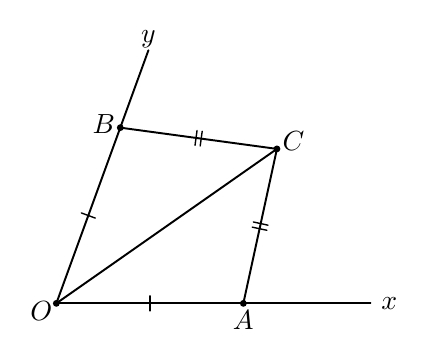
\begin{tikzpicture}[scale=0.95,line cap=round,line join=round]
  \draw[line width=0.7pt] (0.000,0.000) -- (4.200,0.000);
  \draw[line width=0.7pt] (0.000,0.000) -- (1.231,3.383);
  \draw[line width=0.7pt] (0.000,0.000) -- (2.949,2.065);
  \draw[line width=0.7pt] (2.500,0.000) -- (2.949,2.065);
  \draw[line width=0.7pt] (0.855,2.349) -- (2.949,2.065);
  \draw[line width=0.5pt] (1.250,-0.100) -- (1.250,0.100);
  \draw[line width=0.5pt] (0.521,1.140) -- (0.334,1.209);
  \draw[line width=0.5pt] (2.815,0.977) -- (2.619,1.019);
  \draw[line width=0.5pt] (2.830,1.045) -- (2.634,1.088);
  \draw[line width=0.5pt] (1.854,2.113) -- (1.881,2.311);
  \draw[line width=0.5pt] (1.923,2.103) -- (1.950,2.301);
  \node[anchor=west,inner sep=1pt] at (4.300,0.000) {$x$};
  \node[anchor=center,inner sep=1pt] at (1.231,3.533) {$y$};
  \fill (0.000,0.000) circle (1.3pt);
  \node[anchor=center,inner sep=1pt] at (-0.200,-0.100) {$O$};
  \fill (2.500,0.000) circle (1.3pt);
  \node[anchor=center,inner sep=1pt] at (2.500,-0.220) {$A$};
  \fill (0.855,2.349) circle (1.3pt);
  \node[anchor=center,inner sep=1pt] at (0.635,2.399) {$B$};
  \fill (2.949,2.065) circle (1.3pt);
  \node[anchor=center,inner sep=1pt] at (3.169,2.165) {$C$};
\end{tikzpicture}
\end{center}

\end{document}
